\documentclass[bachelor,german]{algothesis}
% possible types: bachelor, master, zula (seminar, practical)
% Für Seminararbeiten und Praktikumsberichte die Vorlage my-seminar-praktikum.tex verwenden!
% possible languages: english, german

\usepackage[utf8]{inputenc}
\usepackage[T1]{fontenc}
\usepackage{lmodern}

\graphicspath{{figures/}}


%%%%%%%%%%%%%%%%%%%%%%%%%%%%%%%%%%%%%%%%%%%%%%%%%%%%%%%%%%%%%%%%%%%%%%%%%%
%%%%%%%%%%%%% Bitte nur ab hier Änderungen vornehmen %%%%%%%%%%%%%%%%%%%%%

\title{Titel der Arbeit} % Geben Sie hier den Titel Ihrer Arbeit an.

\author{Maxi Musterle} % Geben Sie Ihren Namen an.

\newcommand{\abgabedatum}{TT. Monat 20YY} % Hier wird das Abgabedatum angepasst

\supervisors{% Geben Sie die Namen aller Betreuenden an, getrennt durch das Makro '\and'
Jun.-Prof.\ Dr.\ Philipp Kindermann \and
Dr.\ Be TreuerInZwei \and
Be TreuerInDrei, M.\,Sc.
} 


\begin{document}

\begin{abstract}
	Bachelor- und Masterarbeiten bedürfen einer Zusammenfassung.
\end{abstract}

%\begin{germanabstract}
	% If you write in English, but also want to write a German summary, use this command.
%\end{germanabstract}


\thesistableofcontents




%%%%%%%%%%%%%%%%%%%%%%%%%%%%%%%%%%%%%%%%%%%%%%%%%%%%%%%%%%%%%%%%%%%%%%%%%%%%%%%%
\chapter{Einleitung}
Abschlussarbeiten in der Algorithmik sollen in dieser \LaTeX{}-Vorlage erstellt werden.
Dazu stellt die DocumentClass (erste Zeile) Parameter für die verschiedenen Arbeitsformen
(\verb+bachelor, master, zula+) 
zur Verfügung.
Für Seminararbeiten und Praktikumsberichte sollte stattdessen die Vorlage (\verb+algo-seminar-praktikum.tex+) verwendet werden.

The localization of table of content, PDF bookmarks and such can be changed documentwide using the \verb+english+ parameter.


\section{Git}
Falls nicht schon erledigt, sollte auf dem \href{https://gitlab.uni-trier.de/}{Uni Trier GitLab} ein Repository mit dem Namen des Abschlussarbeitstypes sowie Ihrem Namen (also z.B.\ ``bachelorthesis-maxi-musterle'') angelegt werden. Der Ordner Ihrer Abschlussarbeit sowie eventuell Code und Daten sollten dort abgelegt und (spätestens zu Treffen) auf dem Laufenden sein. 
Dieser Vorlage liegt außerdem eine Datei namens \verb+.gitignore+ bei, welche \texttt{git} davon abhält \LaTeX{}-Hilfsdateien mit ins Repository zu schieben. 
Sollten Sie weitere Dateien im Repositoryordner ablegen, welche nicht für alle gedacht sind und daher nicht hochgeladen werden sollten, können sie die Dateinamen oder Ordner dort hinzufügen. 



\subsection{Umgebungen}
Wer bei uns eine Arbeit schreibt, kommt um Definitionen, Sätze, Beweise, Abbildungen und Tabellen nicht herum.

\dots

\begin{definition}
  Dies ist eine \emph{Definition}, welche sich sehr leicht erstellen lässt.
\end{definition}

Eine kurze Überleitung von einer Definition zu einem Satz hilft dem
Leser zu verstehen, wohin die Reise gehen soll.

Manchmal braucht man auch noch ein Lemma, damit der Beweis dann leichter von der Hand geht.

\begin{lemma}[Andres Lemma] % Beachte, dass man sowohl Lemmata als auch Sätzen in der Regel aber keine Namen gibt
 Ein Lemma vorneweg erleichtert die Beweisführung.
 \label{lem:andre}
\end{lemma}
\begin{proof}
 Nach dem Distributivgesetz gilt:
 
 \[ (a+d) \cdot c = ac + dc \]
\end{proof}

\begin{theorem} \label{thm:hauptsatz}
  Wichtige und grundlegende Sätze lassen sich leicht hervorheben.
\end{theorem}
\begin{proof}
  Der Satz gilt offensichtlich, denn nach \cref{lem:andre} gilt:
  \begin{equation*}
    \sum_{i = 1}^{n} 1 = n
  \end{equation*}
  Zudem wird der Beweis automatisch mit einem q.e.d.-Symbol\footnote{Nach Möglichkeit sollte vermieden werden, dass der Beweis mit einer Leerzeile abgeschlossen wird, so wie es beim Beweis von \cref{lem:andre} der Fall ist. Das kann zum Beispiel durch Hinzufügen einer Floskel wie "`Damit ist die Aussage des Satzes bewiesen."' errreicht werden. Übrigens funktionieren Fußnoten genau so. Wichtig ist hier, dass direkt vor dem Kommando kein Leerzeichen oder eine Leerzeile ist.} beendet.
\end{proof}

Auch wenn wir \cref{lem:andre} und \cref{thm:hauptsatz} einen Namen verpasst haben, macht man das in der Regel aber eher nicht.

\begin{corollary}
 Aus einem Satz lassen sich oft einfache Resultate ableiten, die dann in einem Korollar festgehalten werden.
\end{corollary}


\subsection{Verweise}
Auf Sätze, wie z.B.\ \cref{thm:hauptsatz}, lässt sich mithilfe des Befehls \verb+\cref{labelname}+ verweisen, wenn man in der Satz-Umgebung einen "`Label"' mit \verb+\label{labelname}+ gesetzt hat.  
Genauso können wir auf den nächsten Abschnitt, also \cref{sec:leichtigkeit}, verweisen. Ist ein Verweis besonders weit weg, kann man \verb+\cpageref{labelname}+ verwenden, 
um dem Leser zu sagen, auf welche Seite er springen muss -- \cref{sec:leichtigkeit} ist auf \cpageref{sec:leichtigkeit}.
Wir benutzen hier das Paket (\verb+cleveref+), welches nicht nur die Nummer sondern auch automatischen das richtige Label hinzufügt. Benötigt man nur die Nummer, so verwendet man \verb+\ref{labelname}+ .
Üblicherweise beginnt man einen Labelnamen mit dem Typ der Umgebung, auf die man verweist, also z.B.\ \verb+\label{fig:trapez}+ für eine Abbildung (engl.\ \emph{figure}).  
Ach ja, zum Hervorheben (engl.\ \emph{emphasize}) eines \emph{neuen Begriffs} verwendet man den Befehl \verb+\emph{neuer Begriff}+, wenn der neue Begriff zum ersten Mal verwendet wird.


\subsection{Floatende Elemente}
\label{sec:leichtigkeit}
Floatende Elemente (oder auch kurz einfach \emph{floats}) \emph{gleiten} durch das Dokument und \LaTeX{} ermittelt selbstständigt eine geeignete Stelle im PDF um diese Anzuzeigen.
Die wichtigsten floats sind Abbildungen (\verb+figure+), Algorithmen (\verb+algorithm+) und Tabellen (\verb+table+).

In diesem Abschnitt erläutern wir die einzelnen float-Elemente.
Eine Übersicht über die verschiedenen floating-Regeln findet sich am Ende in \cref{tab:floatparameters}.

\subsubsection{Abbildungen}
Abbildungen, wie z.B.\ \cref{fig:trapez}, sind schnell eingefügt.  
\emph{Wichtig:} Fügen Sie eine Abbildung immer erst nach der ersten Referenz auf die Abbildung ein!

\begin{figure}[h] % oft benutzt man einfach die Kombination [htb]
  \centering
  \includegraphics[page=3]{trapez}
  \caption{Das ist eine Abbildung. Sie floatet nach der Regel \emph{here} (h), d.h. \LaTeX{} wird versuchen die Abbildung möglichst direkt vor dem untigen Absatz ("`Im Allgemeinen\dots"') zu platzieren. Weitere Positionierungsregeln werden in \cref{tab:floatparameters} erläutert.} 
  \label{fig:trapez}
\end{figure}

Im Allgemeinen braucht man die Endung der Bilddatei beim Einbinden mit dem Paket \verb+\includegraphics+ nicht mit anzugeben.  
Es empfiehlt sich, alle Bilddateien in einen Unterordner abzulegen.  
In mehrteilige Abbildungen kann man mit dem Paket \verb+subcaption+ jede mit einer eigenen Bildunterschrift versehen.  
Man kann sich dann im Text sowohl auf die Teilabbildungen (z.B.\ \cref{fig:trapez-eins}) als auch auf die Gesamtabbildung (z.B.\ \cref{fig:zwei-trapeze}) beziehen.

Bei Abbildungen ist die Caption üblicherweise unter der eigentlichen Grafik.
Für alle floats gilt, dass das \verb+\label{...}+ direkt nach der \verb+\caption{...}+ gesetzt wird, damit bei einem Click auf die Referenz (\verb+\cref{...}+) auch an die richtige Stelle gesprungen wird (und nicht etwa auf den Absatz darüber).

\emph{Wichtig:} Man sollte sich im Text auf jede Abbildung wenigstens einmal beziehen. 

\begin{figure}[bp]
  \begin{subfigure}{.48\textwidth}
    \centering
    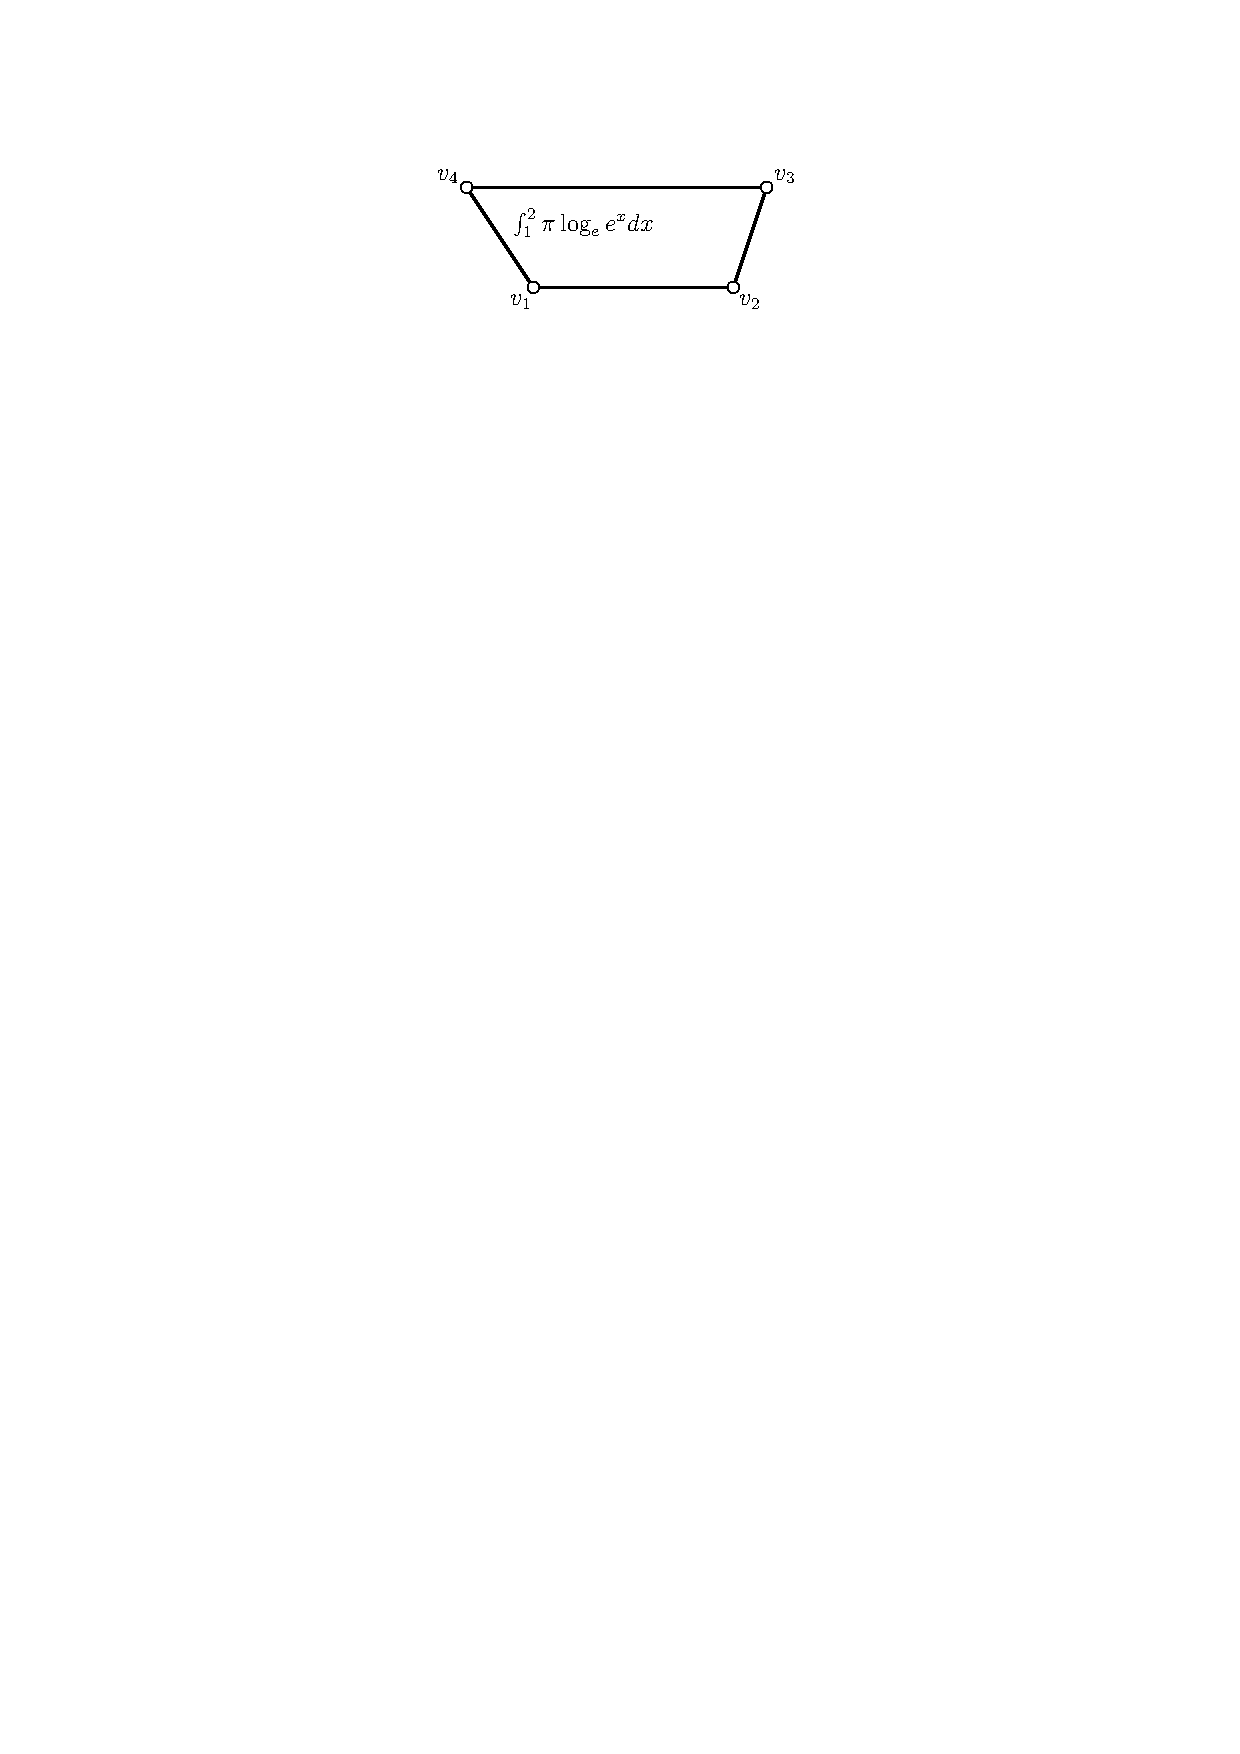
\includegraphics[page=1]{trapez}
    \caption{Die erste Teilabbildung.}
    \label{fig:trapez-eins}
  \end{subfigure}
  \hfill % \hfill sorgt dafür, dass die obere Abbildung an den linken Rand rutscht und die untere Abbildung entsprechend an den rechten. Dies geht nur, weil hier keine Leerzeilen sind (die neue Absätze definieren würden).
  \begin{subfigure}{.48\textwidth}
    \centering
    \includegraphics[page=2]{trapez}
    \caption{Die zweite Teilabbildung.}
    \label{fig:trapez-zwei}
  \end{subfigure}
  \caption{Das ist eine Abbildung, die aus zwei Teilen besteht. Sie versucht erst \emph{bottom} platziert zu werden, an sonsten erzeugt sie eine \emph{float page}.}
  \label{fig:zwei-trapeze}
\end{figure}

\subsubsection{Algorithmen} 
Mit der \verb+algorithm+-Umgebung (aus dem Paket \verb+algorithm2e.sty+) ist es nicht schwer ist Algorithmen in Pseudocode zu setzen, siehe \cref{alg:binsearch}.

\begin{algorithm}[t]
  \SetKw{True}{true}
  \SetKw{False}{false}
  \caption{BinäreSuche(Feld $A$, ganze Zahl $n$, Element $x$)}
  \label{alg:binsearch}
  \Input{sortiertes Feld $A$, Länge $n$, gesuchtes Element $x$}
  \Output{\True genau dann, wenn $x$ in $A$ enthalten ist}
  
  $l = 0$ \;
  $r = n-1$ \;
  
  \While{$l \le r$}{
    $m = \lfloor (l + r)/2 \rfloor$ \;
    \If{$A[m] == x$}{
      \Return \True \;
    }
    \ElseIf{$x < A[m]$}{
      $r = m - 1$ \;
    }
    \Else{
      $l = m + 1$ \;
    }
  }
  \Return \False
\end{algorithm}

Das gleiche geht problemlos auch ohne Zeilennummern, dazu benutzt man einfach in der \verb+algorithm+-Umgebung den Befehl \verb+\LinesNotNumbered+.

\subsubsection{Tabellen}

Um \LaTeX{} etwas in seiner Entscheidung zu beeinflussen haben wir die Möglichkeit, für jedes float einen oder mehrere Positionierungsparameter anzugeben.
Eine Übersicht findet sich in \cref{tab:floatparameters}.

\begin{table}[tb]
 \caption{Positionierungsparameter für floats. Diese Tabelle selbst hat die Wahl zwischen \emph{top} und \emph{bottom}.}
 \label{tab:floatparameters}
 \centering
 \begin{tabularx}{0.9\textwidth}{p{1cm}cX}
  & Wert & Erklärung\\
 \hline
  \texttt{[t]}  & \emph{top} & Das Element wird oben auf einer Seite angezeigt. \\
  \texttt{[b]}  & \emph{bottom} & Das Element wird unten auf einer Seite angezeigt. \\
  \texttt{[p]}  & \emph{page} & Das Element wird auf einer neuen Seite angezeigt. Diese Seite wird auch \emph{float page} genannt; sie kann mehrere \texttt{[p]}-Elemente beherbergen. \\
  \texttt{[h]}  & \emph{here} & Das Element wird nah an der Stelle angezeigt, an der es im Code definiert ist. Das kann irgendwo auf der Seite sein. \\
 \end{tabularx}
\end{table}

Innerhalb der eigentlichen ``Tabelle'' befindet sich ein \verb+tabularx+-Element, dass den Inhalt darstellt.
Elemente dieses Typs haben diverse Vorteile gegenüber normalen \verb+tabular+-Elementen.
Zum einen lässt sich die Breite der Tabelle festlegen (hier $90\%$ der Textbreite), zum anderen stehen neben den klassischen zentrierten, links- oder rechtsbündigen (\verb+l,r,c+) Spalten auch Spalten mit fester Breite zur verfügung.
Diese finden auch in \cref{tab:floatparameters} Verwendung. 
Besonders zu beachten ist, dass sich Text in \verb+p+ oder \verb+X+ Spalten wie text in normalen Text-Absätzen verhält, also mit automatischem Zeilenumbruch und Silbentrennung.

\subsection{Literaturverweise}

Auch Verweise auf andere Arbeiten, wie die von Mustermann und Musterfrau \cite{mustermann+etal-11}, sind ganz einfach.  
Wenn es von einem Artikel eine Konferenzversion \cite{bdln-lhod-02} und eine Zeitschriftenversion \cite{bdln-odgvel-05} gibt, so sollten Sie stets die Zeitschriftenversion (oder ein Buch \cite{gj-cigtn-79}) zitieren.
Tragen Sie bei einem Konferenzartikel neben Titel, Namen der Autoren und des Tagungsbandes gegebenenfalls auch die Namen der Herausgeber in die bib-Datei ein. 
ISBN-Nummern sind nicht nötig.  
Eine große Hilfe beim Identifizieren eier Quelle ist der Digital Object Identifier%
\footnote{\href{https://www.doi.org/}{https://www.doi.org/}}
-- kurz \emph{DOI} genannt.
Sofern möglich sollte stets der DOI einer zitierten Arbeit angegeben werden.
Seien Sie vorsichtig mit Umlauten \cite{bkns-blol-10} und Unterstrichen in der bib-Datei.

\emph{Wichtig:} Zitieren Sie so, dass der Satz, in dem ein Zitat vorkommt, auch ohne das Zitat noch Sinn ergibt; 
das Zitat soll eine Zusatzinformation sein. 
\begin{description}
\item{Gut:} Binucci et al.\ \cite{bdln-odgvel-05} beschäftigen sich mit der Beschriftung von Graphen.  
\item{Schlecht:} \cite{bdln-odgvel-05} beschäftigt sich mit der Beschriftung von Graphen.
\end{description}

Möchte man einen clickbaren Link auf eine Website, wie zum Beispiel \href{https://www.openstreetmap.de/}{OpenStreetMap} oder \href{http://www.graphdrawing.org/}{http://www.graphdrawing.org/} setzen, verwendet man einfach \verb+\href{link}{name}+.

\subsection{Geladene Pakete}
Folgende Pakete werden von der Klasse \verb+algothesis+ automatisch mittels \verb+\usepackage+ geladen:
\begin{itemize}
 \item \verb+[font=small,format=hang,labelfont=bf,figurename=Fig.,tablename=Tab.]{caption}+
 \item \verb+[linesnumbered,algoruled,longend,vlined]{algorithm2e}+
 \item \verb+{amsmath,amsfonts,amssymb,amsthm}+
 \item \verb+{graphicx,xcolor}+
 \item \verb+[bookmarks,bookmarksnumbered,pdfusetitle,pdfencoding=auto]{hyperref}+
 \item \verb+[labelfont=normalfont]{subcaption}+
 \item \verb+{enumerate}+
\end{itemize}

Um ein einheitliches Aussehen der Abschlussarbeiten zu gewährleisten, sollte an diesen Parametern nichts geändert werden.


\section{Fallstricke}
\label{sec:notes}
Einige Sachen sollte man im \LaTeX{}-Code vermeiden, um ein gut gesetztes Dokument zu erhalten. 
Schauen Sie sich dafür bitte auch die Schreibkonventionen an, welche im Ordner mit den Leitfäden zu finden sind.

In \cref{tab:badbox} sehen wir eine klassische \emph{badbox}, also ein Element das zu klein für dessen Inhalt ist.
Mit einer Spalte vom Typ \verb+p+ oder \verb+X+ wäre das nicht passiert.

\begin{table}[h]
 \caption{Der Inhalt einer Tabelle sollte mit Bedacht gewählt werden.}
 \label{tab:badbox}
 \begin{tabular}{ll}
 \hline
  Hier ein kleines Beispiel: &
  Dieser Text wird sehr lang, wahrscheinlich sogar zu lang für eine Zeile. So können Teile des Texts nicht nur über die Tabelle sondern auch über die Seite hinausragen.\\
  \hline
 \end{tabular}
\end{table}

Auch unschön sind Zeilenumbrüche in Formeln, die sich im Fließtext befinden. 
$G=(V,E)$ ein Graph ist ein klassisches Beispiel dafür.
Zu allem Überfluss fängt der vorherige Satz auch noch mit Formelsatz an -- besser wäre ``Sei $G=(\dots$'' gewesen.
Möchte man verhindern, dass Formeln umgebrochen werden, setzt man ihren Inhalt in geschweifte Klammern.

Packt man den Inhalt in geschweifte Klammern, bleibt alles in einer Zeile. 
Sei ${G=(V,E)}$ ein Graph ist ein klassisches Beispiel dafür.
Achtet man nun aber genau auf den rechten Rand dieses Absatzes, so sieht man, dass die Formel über den Rand des Blocksatzes hinausragt -- wir können also das selbe Problem wie oben haben.

In beiden Fällen hilft oft ein einfaches Umstellen der Satzbausteine oder ein kurzes Füllwort.

Setzt man eine Fußnote nach einem Whitespace 
\footnote{Whitespaces sind insbesondere Zeilenumbrüche und Leerzeichen.}, erhält man einen unschönen Abstand zwischen der Markierung und dem Wort, auf das sich die Fußnote wahrscheinlich bezieht.

Punkte sind nicht immer Satzenden, und das sollte man \LaTeX{} auch mitteilen!
Es gibt einen typographischen Unterschied zwischen \verb+Jun.-Prof. Kindermann+ und \verb+Jun.-Prof.\ Kindermann+, der besonders beim Reservieren von Platz sichtbar wird.

Möchte man verhindern, dass Wort und Referenz-Link in unterschiedlichen Zeilen laden, sollte man statt eines normalen Leerzeichens eine Tilde (\verb+~+) verwenden.

Zum Schluss noch der Hinweis, dass die Abschlussarbeit \emph{beidseitig} gedruckt werden soll.

%%%%%%%%%%%%%%%%%%%%%%%%%%%%%%%%%%%%%%%%%%%%%%%%%%%%%%%%%%%%%%%%%%%%%%%%%%%%%%%%
\clearpage
\bibliographystyle{mybabalpha-fl}
\bibliography{mybib}


\end{document}
